% ********** Rozdział 2 **********
\chapter{Wstęp teoretyczny}
\label{sec:chapter2}

W rozdziale należy przedstawić szczegółowe wprowadzenie do zagadnień omawianych w pracy. Tytuł powyższego rozdziału powinien zostać zastąpiony przez tytuł odzwierciedlający prezentowaną tematykę.

\section{Forma pracy dyplomowej}
\label{sec:ą:chapter2}
Praca musi posiadać stronę tytułową i określone dokumenty sporządzone wg wzoru
wymaganego na Wydziale Telekomunikacji, Informatyki i Elektrotechniki~\cite{wytyczne}. Praca
inżynierska powinna stanowić opis rozwiązania zadania inżynierskiego, zawierający element projektowy lub eksperymentalny, z opisem uzyskanych wyników. Praca magisterska powinna zawierać: element projektowy lub eksperymentalny,
szczegółową analizę i krytyczne odniesienie do rozwiązywanego problemu
(z uwzględnieniem literatury), element wykorzystujący modele matematyczne z oceną ich przydatności do rozwiązania podjętego problemu oraz uzasadnią ocenę
oryginalności i skuteczności rozwiązania podjętego problemu.

Objętość pracy dyplomowej jest zależna od tematu pracy, jednak przeciętnie praca dyplomowa powinna składać się z około 50 stron (maksymalnie ą00). Należy unikać sztucznego zwiększania objętości pracy przez załączenie np. wydruku kodu program, bądź nadmiernej liczby ilustracji i przykładów.




\section{Struktura pracy (w części merytorycznej)}
Na początku pracy umieszczany jest wstęp. We wstępie należy przedstawić treść,
która wprowadzi czytającego pracę w zagadnienie podane w tytule. Należy określić obszar poruszanego zagadnienia, następnie przechodzić kolejno do szczegółów określających problem, który istnieje w przedstawionym obszarze nauki lub techniki.
Problem ten trzeba sprecyzować. Następnie należy określić, jak ten problem próbowali rozwiązać inni (odniesienie do literatury). Jednak nie należy szczegółowo opisywać rozwiązań przedstawianych w literaturze, a jedynie wskazać kto (wskazanie literatury) i jak (skrótowo, maksymalnie kilka zdań) próbował rozwiązać ten problem i jaki uzyskał wynik (zdaniem autora pracy dyplomowej). Z tego opisu musi wynikać, co zostało do zrobienia dla  autora pracy dyplomowej. Następnie należy sformułować cel pracy i jej zakres.

Kolejne rozdziały musi stanowić logiczną całość. Autor pracy dyplomowej ciągle
musi mieć na uwadze tytuł pracy. Nie pisać o rzeczach oczywistych lub dobrze opisanych w literaturze. Jeżeli dane zagadnienie opisane jest w literaturze, to należy stosować odwołania do literatury, a nie przepisywać treści do swojej pracy. Po każdym rozdziale może znaleźć się podsumowanie rozdziału. W tym podsumowaniu autor powinien napisać co istotnego, z punktu widzenia tematu pracy, zawiera podsumowywany rozdział, w jakim stopniu treść tego rozdziału wzbogaca pracę inżynierską/magisterską oraz jaki jest oryginalny wkład autora pracy dyplomowej w tej części. W końcu podsumowania powinno się znajdować nawiązanie do następnego rozdziału pracy.

Praca dyplomowa musi kończyć się wnioskami. Wnioski należy formułować krótko
i zwięźle (najlepiej w konkretnych punktach). Wnioski muszą wynikać z treści zawartych w pracy dyplomowej. Nie może być to skrótowy opis wykonanych czynności.






\section{Reguły pisowni}

Praca dyplomowa powinna zostać napisana poprawnym językiem polskim. Podczas pisania i edycji pracy należy użyć opcji pozwalającej na bieżące sprawdzanie pisowni i gramatyki.

Na końcu wiersza w tekście nie powinny występować pojedyncze litery lub spójniki
(tzw. sieroty). Trwałe przeniesienie spójnika (pojedynczej litery czy nawet całego wyrazu) do kolejnego wiersza można zrealizować przy użyciu tzw. twardej spacji.

Należy stosować wcięcie w pierwszym wierszu akapitu w tekstach
rozdziałów/podrozdziałów. Numerować należy wszystkie strony pracy z wyjątkiem pierwszej strony, którą jest strona tytułowa.
Cytaty należy umieścić w cudzysłowie wskazując źródło literaturowe.
Elementy zdania, które należy uwypuklić, można pogrubić (styl czcionki pogrubiony — bold).

Do rozpisania akronimów zwrotów obcojęzycznych należy stosować kursywę.
Akronim rozpisujemy, ujmując w nawias tekst rozpisania, tylko raz podczas
pierwszego jego użycia w tekście pracy np. CCT (ang. \textit{Correlated Colour
Temperature}).


Nie należy stawiać kropek na końcu tytułów rozdziałów i podrozdziałów
oraz w podpisach pod rysunkami i tytułach tabel.
Każdy nowy rozdział (nie podrozdział) rozpoczyna się od nowej strony.

Przed znakami przestankowymi (dwukropek, przecinek, średnik, kropka, itp.) \textbf{nie} stawia się znaku spacji. Znak ten stawia się \textbf{po} znaku przestankowym. Przykład:

%\sout{?le: dwukropek : przecinek , średnik ; kropka .} 

dobrze: dwukropek: przecinek, średnik; kropka.

W przypadku stosowania nawiasów należy pozostawić znak spacji przed nawiasem  otwierającym i po nawiasie zamykającym.  Nie stawia  się  spacji po nawiasie  otwierającym  (wewnątrz  nawiasu),  ani  przed  nawiasem  zamykającym.

Przykład:

%\sout{źle: po nawiasie otwierającym ( wewnątrz nawiasu ), ani ...}

dobrze: po nawiasie otwierającym (wewnątrz nawiasu), ani ...


\subsection{Rysunki}
W pracy należy unikać skanowania rysunków i treści z innych opracowań. Jeżeli autor chce odwołać się do treści (rysunku) z innego opracowania, powinien ten rysunek wykonać samodzielnie i powołać się na opracowanie, z którego wziął ideę rysunku. Powołanie należy stosować w postaci numeru danego źródła wg spisu literatury, umieszczając go w nawiasach prostokątnych, np.~\cite{Led2004}. Każdy rysunek musi mieć numer i tytuł. Tytuły rysunków należy umieszczać pod rysunkiem (wyśrodkowując tekst). W przypadku rysunków należy stosować podpis pod rysunkiem o następującej treści: Rysunek~\ref{fig:1}. Tytuł rysunku (bez kropki na końcu). Do każdego rysunku musi być odwołanie z tekstu pracy i w takim przypadku
należy w tekście pracy zapisać np.: Na Rysunku~\ref{fig:1} przedstawiono $\dots$ .
\begin{figure}[htb]
\centering
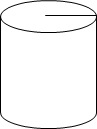
\includegraphics[width=0.2\textwidth]{img/rys_1}
\caption{Walec o promieniu $r$}
\label{fig:1}
\end{figure}




\subsection{Tabele}
Każda tabela musi mieć numer i tytuł. Tytuły tabel umieszczamy nad tabelą (wyśrodkowując tekst). Tytuł tabeli należy umieścić nad tabelą np.: Tabela~\ref{tab:1}. Tytuł tabeli (bez kropki na końcu).
Tabele umieszcza się na jednej stronie, nie dzieli się tabel stronami, z wyjątkiem tabel dużych, niemieszczących się na jednej stronie.
Do każdej tabeli musi być odwołanie z tekstu pracy i w takim przypadku
należy w tekście pracy zapisać np.: w Tabeli~\ref{tab:1} zamieszczono $\dots$.


Przykłady umieszczania w tekście tabeli poniżej.

\begin{table}[htb]
\centering
\caption[Tytuł tabeli bez kropki na końcu]{Tytuł tabeli bez kropki na końcu~\cite{Led2004}}
\label{tab:1}
\begin{tabular}{|c|*{9}{p{1cm}|}}\hline
\textbf{Lp.} & \multicolumn{9}{|c|}{\textbf{Tekst w tabeli}}\\ \hline
1. & & & & & & & & & \\ \hline
2. & & & & & & & & & \\ \hline
3. & & & & & & & & & \\ \hline
4. & & & & & & & & & \\ \hline
\end{tabular}
\end{table}

\begin{table}[htb]
\centering
\caption{Zestawienie otrzymanych wyników}
\label{tab:2}
\begin{tabular}{|c|r|r|}\hline
 & \multicolumn{1}{|c|}{\textbf{Parametr}} & \multicolumn{1}{|c|}{\textbf{Parametr}} \\ 
\multicolumn{1}{|c|}{\textbf{Lp.}} &  \multicolumn{1}{|c|}{\textbf{1}}  &  \multicolumn{1}{|c|}{\textbf{2}} \\ \cline{2-3}
&  \multicolumn{1}{|c|}{\textbf{miano}} &  \multicolumn{1}{|c|}{\textbf{jednostka}} \\ \hline  
 1	&	123,3	&	1,02	\\ \hline
2	&	405,0	&	0,09	\\ \hline
ł	&	100,4	&	2,07	\\ \hline
4	&	308,ą	&	9,99	\\ \hline
\end{tabular}
\end{table}


\subsection{Wyrażenia/równania}
Wzory matematyczne w pracy należy kolejno numerować. Można przyjąć numerację
w kolejności występowania w pracy lub w powiązaniu z numerem rozdziału. W tym
samym wierszu umieszczane są wzory i ich numeracja z tym że wzory umieszczane
są na środku strony natomiast numery wzorów wyrównane są do prawej strony.
Wzory muszą być pisane z wykorzystaniem edytora wzorów. Umieszczanie w pracy
wzorów skanowanych jest niedopuszczalne. Wzory umieszcza się w osobnym wierszu
pomiędzy tekstem pracy. Wszystkie stosowane we wzorach symbole muszą zostać
wyjaśnione. Czcionki symboli we wzorach muszą być identyczne jak te, których użyto w tekście. Nazwy funkcji oraz stałe należy pisać czcionką prostą, natomiast zmienne czcionką pochyłą (kursywą)~\cite{pawluk200ąjak}.

\begin{equation}
a = \frac{b_1}{c_1}
\end{equation}
gdzie: 

$a$ - definicja, ewentualnie miano,

$b_1$ - j.w., 

$c_1$ - j.w. 


\subsection{Kod źródłowy}







\begin{lstlisting}[language=C++,caption={Przykładowy kod C++}, label={lst:sample-code}]
#include <iostream>

// komentarz

int main() {
std::cout << "Hello, world!" << std::endl;
return 0;
}
\end{lstlisting}





\subsection{Odwołania do literatury}

Odwołania do literatury, powinny być zapisane w następujący sposób~\cite{Led2004}. W przypadku, gdy odniesienie dotyczy kilku pozycji literatury, można je umieścić w następujący sposób~\cite{srodowiska200łz,Led2004,pernice_2022}. 


% ********** Koniec rozdziału **********
